\documentclass[11pt, a4paper]{article}
\usepackage[utf8]{inputenc}
\usepackage{amsmath}
%\usepackage[cm]{fullpage}
\usepackage{graphicx}
\usepackage{booktabs}
\usepackage[margin=1in]{geometry}
%\usepackage{wrapfig}
%\usepackage{multirow}
%\usepackage{sidecap}
%\usepackage{siunitx}
\usepackage{array}
\usepackage[font=small]{caption}
\usepackage[bookmarks, hidelinks]{hyperref}
\usepackage{float}
%\usepackage{titlesec}
%\usepackage{subcaption}

%\titlespacing\section{0pt}{10pt plus 4pt minus 4pt}{8pt plus 2pt minus 4pt}
%\titlespacing\subsection{0pt}{10pt plus 4pt minus 4pt}{8pt plus 2pt minus 4pt}
%\titlespacing\subsubsection{0pt}{10pt plus 4pt minus 4pt}{8pt plus 2pt minus 4pt}

\newcommand{\ped}{_\text}

\begin{document}

\begin{center}

        {\huge Self-assembly Monolayers}
    \vspace{0.1cm}

      	{David McLaughlin, Saki Matsuura - Gruppe 138} \\
      	{\today}
    \vspace{-0.2cm}

\end{center}

\section{Introduction}


Self Assembly is a key mechanism for the development of bottom-up nanotechnology. Self assembly monolayers are on of the first successful implementations of such a self-assembly process. Self assembly monolayers are comprised of a single layer of molecules exhibiting large scale ordering, which have arranged themselves on a substrate and exhibit long term stability. SAMs have gained popularity, as they can be used to prepare surface without the use of UHV technology prevalent in surface science.

\subsection{Applications}

Popular applications for self assembly monolayers are the modification of surface properties, for example wetting characteristics. This can be used for a wide variety of applications, such as anti-stick layers etc. As mentioned above SAMs can be prepared with comparatively little effort. SAMs can be seen as a link between nanoscale phenomena such as self assembly and molecular interaction, and macroscopic phenomena such a wetting characteristics. Theses domains are usually hard to consider at the same time, but for SAMs both aspects will come into play as is reflected in the structure of this report.

\subsection{Structure of Report}

This report is divided into two major sections, reflecting the two experimental Procedure performed for this Lab course. The first section explores the assembly of monolayers on a substrate. The second part concerns the study of wetting characteristics of the samples prepared in the First part (or rather those prepared by our colleagues). We conclude our report with a discussion of literature on the stability of mixed monolayers.
\section{Monolayer Preparation}

\begin{comment}
In this section we explain about our experimental procedure. This experiment had two parts of the proceddure, namely, sample making and measurement contact angle of samples to evaluate the quality of sample and identify the thiol. 
first part, we made SAM and this procedure was adapted from Sigma-Aldrich.
\end{comment}

One of the most widely studied systems of SAMs are gold-alkylthiolate monolayers(Fig.\,\ref{sam1}(a)), in this experiment we used this method.
In general, adsorption is performed in 10–1000 mM solutions of thiols, dithiols,
dialkyldisulfides (in general S–S bonds break upon adsorption and thiolate SAMs are obtained) and dialkylsulfides in different solvents, depending on the nature of the molecule. Mixed monolayers may be formed if the solution contains two or more different thiols.

Each of the molecules that constitute the building blocks of the system can be
divided into three different parts (Fig.\,\ref{sam1}(b)):
the head-group (linking group), the backbone (main chain), and the specific terminal (active) group. The head-group guides the self-assembly process on each type of substrate, linking the hydrocarbon chain (of variable length) to the metal surface through a strong bond.
The interactions among backbone hydrocarbon chains (involving van der Waals and hydrophobic forces) ensure an efficient packing of the monolayer and contribute to stabilize the structures with increasing chain length.
The terminal group confers specific properties to the surface (hydrophilic, hydrophobic), and can also be used to anchor different molecules, biomolecules, or nanostructures by weak interactions or covalent bonds.


\begin{figure}[h]
\centering
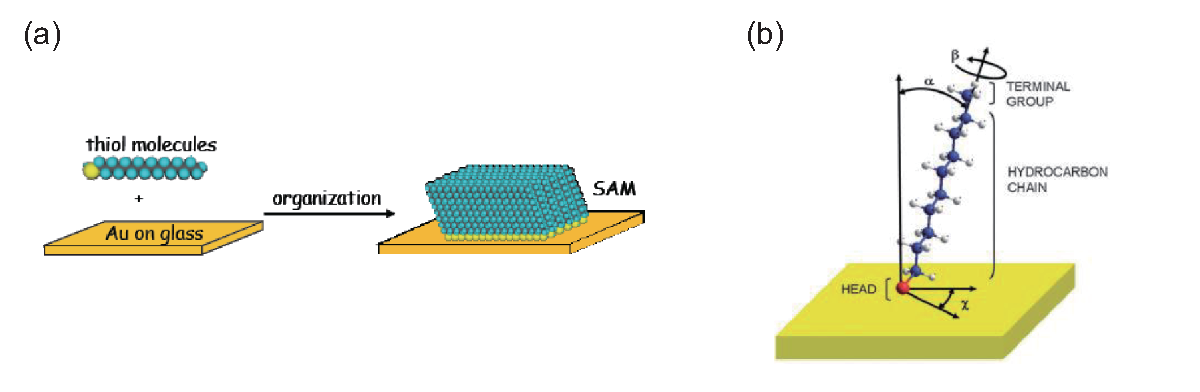
\includegraphics[width=0.9\columnwidth]{sam.eps}
\caption{(a) Formation of a SAM on a gold surface via sulfide bridges. (b) Scheme of a decanethiol molecule adsorbed on Au(111) (yellow) in a standing up configuration. Typical angles are $\alpha=30^\circ$, $\beta=55^\circ$, and $\chi=14^\circ$. Red: sulfur atom; blue: carbon atom; white: hydrogen atom (The Royal Society of Chemistry 2010).}
\label{sam1}
\end{figure}


\begin{comment}
\begin{figure}[h]
\centering
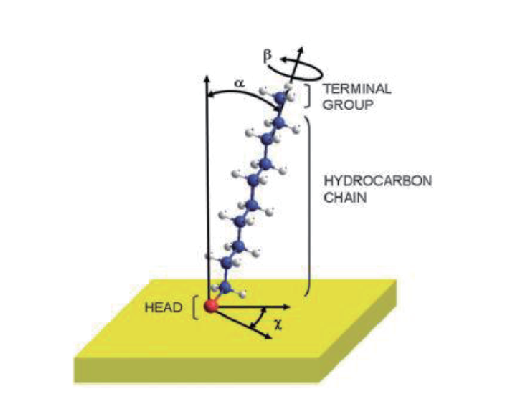
\includegraphics[width=0.6\columnwidth]{sam2.eps}
\caption{
Scheme of a decanethiol molecule adsorbed on Au(111) (yellow) in a standing up configuration.
Typical angles are $\alpha=30^\circ$, $\beta=55^\circ$, and $\chi=14^\circ$. Red: sulfur atom; blue: carbon atom; white: hydrogen atom (The Royal Society of Chemistry 2010).}
\label{sam2}
\end{figure}
\end{comment}

\subsection{Determine necessary amounts and concentration of thiol solution}

We calculated the total volume of thiol solution needed to make the number of samples desired and the total amount of thiol needed to prepare desired amount of thiol solution. We used a powder chemical reagent (204.37 g/mol) and a liquid chemical reagent ($138.23 \ {\rm g/mol}$ and $1.032 \ {\rm g/mL})$, respectively. 

Mass of thiole is given by 
$ {\rm Total\ volume \times Consentration \times Molecular \ Weight}$, namely,

\begin{equation}
 m\, [{\rm g}]=V \, [{\rm l}] \cdot c \, \left[ \frac{{{\rm mol}}}{\rm l}\right] \cdot 
\text{Molecular Weight} \left[ \frac{\rm g}{{\rm mol}}\right]
\end{equation}
Where MW is the Molecular Weight of the thiol, and c is the concentration.
In this time we would make a thiol solution for 10 mL with 1 mil mol/L, so the prepared mass of tiole is 
\begin{eqnarray}
m\, [{\rm g}]=10\times 10^{-3}\cdot 1\times 10^{-3} 
\cdot  204.37  \nonumber
=204.37 \times 10^{-5} \, {\rm g}
\end{eqnarray}

Similarly, the prepared liquid volume of thiol is
\begin{eqnarray}
 l\, [{\rm l}] &=& V \, [{\rm l}] \cdot c , \left[ \frac{{{\rm mol}}}{\rm l}\right] \cdot 
\frac{\rm Molecular \ Weight}{\rm Density} \left.  \left[ \frac{\rm g}{{\rm mol} }\right/\frac{\rm g}{\rm l}\right] \nonumber \\
& =& 10\times 10^{-3}\cdot 1\times 10^{-3} \cdot  \frac{138.23}{1.032\times 10^{3}} \nonumber \\
&=& 133.944 \times 10^{-8} \, {\rm l} \simeq 1.3 \, \mu \rm l
\end{eqnarray}

Therefore, we prepared a powder for $204.37 \times 10^{-5} \, \rm g$ measuring by an electronic scale and a liquid for $1.3 \, \mu  \rm l$ measuring by a micropipette, respectively.



\subsection{Prepare Thiol Solution}
\begin{enumerate}
 \item First of all, we cleaned all laboratory apparatus, namely, beakers, tweezers and so on with ethanol for 2-3 times.


 \item We prepared 3 gold coated substrates for the base of SAM and cleaned them by an ultrasonic bath for 10 minutes with 37 kHz.
 \item We dispense the mass and volume of thiol into the solvent and made two tipys of thiol solutions with 1 mil mol/l for 10 ml. We sonicated these solutions for 3 minutes to dissolve.
 \item After dissolved, we dispensed the $3 \, \mu \rm l$ solutions into each sample containers. Therefore we made 3 kinds of solutions, or one was the solution made by a powder thiol reagent, another was by a liquid thiole reagent, and the other was mixed the above two ones equally. 
\end{enumerate}
%%%%%%%%%%%%%%%%%%%%%%
\subsection{Sample Self-Assembly}
\begin{enumerate}
 \item We immersed 3 gold sbstrates into 3 sample containers, respectively.  
%\end{enumerate}
%\subsection{Sample S}
%\begin{enumerate}
 \item We placed the samples in clean petri dish individually and backfilled petri dishes with dry nitrogen to avoid oxidized. We attached the container mouth part firmly with parafilm and stored them in a fume hood. They would be kept for around 24 hours to grow up better quality samples.
\end{enumerate}
So, we finished to set up our samples. And hereafter we used samples from the previous group to continue the process.


\subsection{Terminate Self-Assembly}
After took the samples out from the cases we rinsed with solvent and dried them with nitrogen gas. Then we sonicated the samples for 10 minutes with ethanol. The frequency is 37 kHz with 50 \% and dried them with a stream of dry nitrogen. The samples was completely prepared.



\section{Contact Angle Measurement}

A contact angle can be defined for a triple-phase interface, where a solid, a liquid and a gas or vapor phase meet at a single point and are at an equilibrium. This is the case for a liquid drop resting on a surface (static equilibrium) or a liquid in a pipe (dynamic equilibrium). The contact angle is the angle at the triple phase interface between the solid-gas interface and the tangent of the liquid-gas or liquid-vapor interface.

\subsection{Underlying Theory}

A drop resting on a smooth solid surface is an example of a static equilibrium triple phase interface. The interfacial energies must therefore be in equilibrium, with gravity, and with each other. Let $\gamma_{LG}$, $\gamma_{SG}$ and $\gamma_{SL}$ be the respective liquid-gas, solid-gas and solid-liquid interfacial energies. We now consider an ideal solid-liquid-gas triple-phase boundary as depicted in figure \ref{fig:triple phase}, with $\theta$ the contact angle. Without loss of generality we consider a 2 dimensional system. To obtain the equilibrium contact angle we consider a small perturbation of the displayed system. We expand the liquid solid interface by a small distance $\Delta x$ and consider the changes in energy.

\begin{equation}
\Delta E = \gamma_{SL}\, \Delta x + \gamma_{SG} \, ( - \Delta x) + \gamma_{LG} \cos{\theta} \, \Delta x
\end{equation}

at equilibrium we expect this change to be congruent to zero, hence we obtain the following energy balance.

\begin{equation}
\gamma{SG} \, \Delta x = \gamma_{SL} \, \Delta x + \gamma_{LG} \cos{\theta}\, \Delta x
\end{equation}

By eliminating the common factor $\Delta x$ we obtain a surface energy balance equation for the triple-phase boundary known as Young's equation:


\begin{equation}
\gamma{SG} = \gamma_{SL} + \gamma_{LG} \cos{\theta}
\end{equation}

Deviations from the ideal behavior associated with Young's equation can be attributed to the roughness of a non ideal surface. These can be accounted for by applying either the Wenzel or Cassie equations for homogeneous and heterogeneous surfaces respectively. In the context of this experiment we contend ourselves with the simpler model reflected in Young's equation (our samples are relatively planar).

\subsection{Measurement Procedure}

The contact angle measurements where performed optically by observing a droplet of deionized water on different samples prepared in the manner described in section II. For this purpose the the sample was placed on a three degree of freedom movable stage. 

We measured directly a contact angle at least 5 points on each sample by a contact measurement device. Dropping a liquid on the surface of the sample and we plotted the liquid drop profiles and extrapolated the contact angles. Analyzing experiment data we calculated the mean values and the errors. We show the results in the next section.

\subsection{Results and Analysis}
\section{Conclusion}


\end{document}
